\documentclass[12pt, letter paper]{report}
\usepackage{graphicx} % Required for inserting images
\usepackage[document]{ragged2e}
\usepackage[a4paper, total={6in, 7in}]{geometry}
\setcounter{tocdepth}{6} 
\setcounter{secnumdepth}{6} 
\setcounter{chapter}{0}
\usepackage{setspace}
\usepackage{blindtext}
\usepackage{layout}
\usepackage[dvipsnames]{xcolor}
\usepackage{biblatex} %Imports biblatex package
\addbibresource{sample.bib} %Import the bibliography file
\usepackage{geometry}
\geometry{
 a4paper,
 total={170mm,257mm},
 left=27mm,
 top=20mm,
 right=27mm,
 }
\title{DBMS MINIPROJECT REPORT }
\author{Akshay}
\date{August 2023}

\begin{document}
\thispagestyle{empty}
%\maketitle
%cover page 
\begin{center}
\Large\textbf{ ST JOSEPH ENGINEERING COLLEGE\\ }
\textbf{An Autonomous Institution}\\
Affiliated to VTU, Belagavi\\
\textbf{Mangaluru-575028}
\end{center}

\begin{figure}[h]
 \centering
 
\includegraphics[scale=1.1]{sjec.jpeg}
 \label{sjeclogo}
\end{figure}

\begin{center}
   \textbf{ MINI PROJECT REPORT ON }
\end{center}
\begin{center}
   \Large\textbf{“TAILOR'S DATABASE”}
\end{center}



 
\begin{center}
   \Large \textbf{Submitted By \\}
\end{center}

\begin{center}
\justifying{
\hspace{3.5 cm}Abhik L Salian\hspace{3.5cm}4SO21CS004\\
%\vspace{0.5 cm}
%XXXXXX\hspace{9.5 cm}4SO21CS403
}
\justifying{

\hspace{2.9 cm}Akshaya Kumar S\hspace{2.9 cm}4SO21CS014
}
\end{center}
   \begin{center}
\large \textbf{\\Under the guidance of \\}
\large  \textbf{ \\Ms Pruthvi  M R\\ }
\large  Assistant Professor,\\ Department of CSE
\end{center}

\vspace{0.5cm}
\begin{center}
\large\textbf{\\ DEPARTMENT OF COMPUTER SCIENCE AND ENGINEERING\\ 2022-2023}

\end{center}
\vspace{2cm}
\thispagestyle{empty}
% certificate Page 
\section*{}
\begin{center}
\Large\textbf{\\ ST JOSEPH ENGINEERING COLLEGE}\\
\end{center}
\begin{center}
\textbf{\textit{An Autonomous Institution}}\\

\large \textbf{Vamanjoor, Mangaluru-575028}\\
\large \textbf{ DEPARTMENT OF COMPUTER SCIENCE AND ENGINEERING} 
\end{center}
\vspace{0.1cm}
\begin{center}
\begin{figure}[h]
 \centering
 
\includegraphics[scale=0.7]{sjec.jpeg}
 \label{sjeclogo}
\end{figure}
\end{center}
\vspace{-1cm}
\begin{center}
\large\textbf{\textcolor{blue}{CERTIFICATE}}
\end{center}
\begin{center}
\justifying{
\large Certified that the project work entitled \textbf{“Tailor's Database”} carried out by }
\end{center}
\begin{center}
\justifying{
\hspace{3.5 cm}Abhik L Salian\hspace{2.62 cm}4SO21CS004
}
\end{center}
\begin{center}
\justifying{
\hspace{3.5 cm}Akshaya Kumar S\hspace{2.1 cm}4SO21CS014
}
\end{center}

\begin{center}
\justifying{
\par{

\large bonafide students of IV semester students in partial fulfillment for the award of Bachelor of Engineering in Computer Science and Engineering of St Joseph Engineering College during the year 2022-23.It is certified that all corrections/suggestions indicated during Internal Evaluation have been incorporated in the report.The project report has been approved as it satisfies the academic requirements in respect of miniproject work .\\\\\\

} 
}
\end{center}
\begin{center}
\justifying{ 
\large\textbf{Ms Pruthvi M R \hspace{5 cm}  Dr Sridevi Saralaya  \\}
\hspace{1cm}\large\textbf{  Project Guide \hspace{6.7 cm} HOD-CSE 
}
}

\end{center}


\thispagestyle{empty}
\newpage
\chapter*{\centering Acknowledgment}
\justifying{
\addcontentsline{toc}{chapter}{\numberline{}Acknowledgment}
% \linespread
  \large The satisfaction and euphoria that accompanies the successful completion of any task would be incomplete without mentioning the people who made it possible, whose constant guidance and encouragement crowned our efforts with success.\\
    \\
    We take this opportunity to thank those who have helped and motivated us throughout the completion of this project.\\
    \\
    We would like to express our deep and sincere gratitude to our project guide, \textbf{Ms Pruthvi M R}, Assistant Professor, Department of Computer Science and Engineering, for her constant guidance and support, without which this project wouldn’t have been completed successfully. \\
    \\ 
    We owe our great debt to \textbf{Dr Sridevi Saralaya}, Head of the Department of Computer Science and Engineering, for her support and encouragement during the course of development of this project. \\
    \\
    We are immensely grateful to our Principal, \textbf{Dr Rio D’Souza}, our Director, \textbf{Rev. Fr Wilfred Prakash D’Souza}, and Assistant Director \textbf{Rev. Fr Kenneth Rayner Crasta} for their support and encouragement. \\
    \\
    We extend our gratitude to the entire faculty and the staff of the Department of Computer Science and Engineering, SJEC, for their advice, kind co-operation and assistance throughout the academic year.\\
    \\
    Lastly, we would like to express our heartfelt appreciation towards our classmates and seniors for their guidance and suggestions.
 
    
 }
%/\thispagestyle{empty}
\pagenumbering{roman}
\chapter*{\centering Abstract}

\justifying{
\addcontentsline{toc}{chapter}{\numberline{}Abstract}
\begin{spacing}{1.5}
In the ever-evolving landscape of fashion and clothing customization, tailors and designers face the challenge of efficiently managing client measurements. This abstract introduces a Tailor's Database, a digital platform designed to empower tailors and clients alike in the process of storing and accessing personalized measurements.

The Tailor's Database is a secure and user-friendly system that offers a convenient and streamlined approach to recording, storing, and retrieving measurements for clients. It leverages technology to enhance the tailoring experience, ensuring accuracy, convenience, and personalization.

Tailors and clients often find themselves grappling with the complexities of managing measurements, but the Tailor's Database seeks to simplify this process. It adopts a client-centric approach, allowing clients to create profiles and securely store their measurements. This not only saves time during fittings but also fosters client loyalty by providing a seamless experience.

The system also facilitates effective communication between tailors and clients. Tailors can access the stored measurements, consult with clients remotely, and provide guidance, resulting in a collaborative and efficient tailoring process. This digital interaction enhances the tailoring experience, making it more engaging and responsive to individual preferences.

In conclusion, the Tailor's Database offers a comprehensive solution for tailors and clients seeking a modern and efficient way to manage measurements. By merging technology with the art of tailoring, it not only improves the accuracy and precision of garments but also enhances the overall client-tailor relationship. This digital platform represents a promising step forward in the ever-evolving world of personalized tailoring, ensuring both clients and tailors benefit from a more seamless and personalized experience.
\end{spacing}
%/\thispagestyle{empty}



%\section*{\centering TABLE OF CONTENT}
%/\thispagestyle{empty}
\renewcommand{\contentsname}{Table of Contents}
\tableofcontents
\addcontentsline{toc}{chapter}{\numberline{}Table of Contents}
\listoffigures
\addcontentsline{toc}{chapter}{\numberline{}List of Figures}
\listoftables
\addcontentsline{toc}{chapter}{\numberline{}List of Tables}
\newpage
%/\tableofcontents
\thispagestyle{empty}
\chapter{Introduction}
\begin{spacing}{1.5}
Amid the digital transformation sweeping industries, the tailoring sector is embracing innovation. This report details the creation of an online tailors' database and e-commerce platform, designed to meet the evolving needs of both tailors and customers. The platform simplifies the process of ordering custom shirts and pants while enabling users to securely manage their measurements.

Traditionally, tailoring has involved in-person visits, manual measurements, and lengthy wait times. This platform bridges tradition with modernity, incorporating user authentication, database management, e-commerce features, and secure payments.

The report offers insights into database design, web development, user interface, security, payment integration, testing, and maintenance. It emphasizes user-friendly design, data security, legal compliance, marketing, and support. This platform represents a forward-thinking approach to modernizing tailoring, offering convenience to users and efficiency to tailors.
\end{spacing}
\section{Problem Definition} 
\begin{spacing}{1.5}
To create a database that can store client’s data like client name, phone number, address, and all the measurements so that the tailor can use the data in the database without having to measure again and again.
\end{spacing}

%\subsection{vvv}
\section{Scope and Importance}
\subsection{Scope:}
The scope of the Tailor's Database for client measurement storage is extensive and encompasses various aspects of the tailoring industry and client-tailor relationships. 
\pagenumbering{arabic}
Key areas within the scope of this topic include:
\begin{spacing}{1.5}
\begin{itemize}
\item\textbf{Measurement Accuracy:} Ensuring precise and accurate measurements to create perfectly fitting garments.

\item\textbf{Client Convenience:} Streamlining the measurement recording process for clients, enhancing their overall experience.

\item\textbf{Data Security:} Implementing robust security measures to protect clients' sensitive measurement data.

\item\textbf{Communication:} Facilitating seamless communication between tailors and clients, regardless of geographical distances.

\item\textbf{Analytics and Business Insights:} Utilizing measurement data for trend analysis, inventory management, and business growth.

\item\textbf{Tailor Collaboration:} Encouraging collaboration among tailors, enabling them to consult and support each other in the tailoring process.

\end{itemize}

\subsection{Importance:}
The Tailor's Database holds significant importance in the tailoring industry for several reasons:
\begin{itemize}
\item\textbf{Enhanced Accuracy:} Accurate measurements are fundamental to creating well-fitting garments, reducing the need for multiple fittings and alterations, thus saving time and resources.

\item\textbf{Client Satisfaction:} Offering a convenient and personalized experience builds client loyalty, leading to repeat business and positive word-of-mouth referrals.

\item\textbf{Data Security: }Safeguarding client measurements instills trust, ensuring clients feel comfortable sharing their personal information.

\item\textbf{Efficiency:} Streamlining measurement management reduces administrative tasks, enabling tailors to focus more on their craft.

\item\textbf{Business Growth:} Leveraging measurement data for analytics and insights can help tailors make informed business decisions and stay competitive in the market.

\end{itemize}
\end{spacing}
\chapter{Software Requirement Specification}

\section{Functional Requirement Specification} 
\begin{itemize}
\begin{spacing}{1.5}
\item The first page that appears while entering the website is the welcome page which consists of 3 buttons namely: Sign Up, Sign In and Tailor Login
\item If you are a new user, you have to first register yourself by clicking on the Sign Up button.
\item After filling all the fields correctly your details will be stored in the database and you will be directed to the sign in page. 
\item After entering correct credentials in sign in page, you will be redirected to home page where you can place order for shirt or pant and can also view your profile details and measurements and can edit your measurements.

\item The admin has access to all the user data.The users will have access to their own data only. 
\item The measurements and all the details that they enter cannot be accessed by other users.
\item The github repository of the codes of our project: \\https://github.com/AbhikSalian/tailor-database
\\
\\
\textbf{Data handling logic:}
\\
The data handling logic of an online tailors' database and e-commerce project involves managing various types of data, including user profiles, measurements, product information, and order details. Here is a breakdown of the key data handling components and their logic:

\item\textbf{User Registration:} When a user registers, their information (name, email, password) is securely stored in the user database.
\item\textbf{Login:} Users can log in by providing their credentials, which are verified against the stored data.
\item\textbf{User Profiles:} Each user has a profile where they can store and manage their measurements and order history.
\item\textbf{Measurement Input:} Users can input and save their body measurements in their profiles.
\item\textbf{Data Validation: }The system validates measurement data to ensure it meets required criteria (e.g., valid measurements).
\item\textbf{Measurement Updates:} Users can update or edit their measurements as needed.
\end{spacing}
\end{itemize}
\section{Software Requirement Specification}
Software Requirement Specification
\begin{itemize}
 \item {\textbf{Language} : HTML, CSS, Java Script, PHP}
 \item {\textbf{Database used}: MySQL}.
 \item {\textbf{Design used}: HTML, JavaScript}.
 \item {\textbf{Operating System}: Window 11}.
 \item {\textbf{Software used}: XAMPP}.
\end{itemize}

\section{Hardware Requirement Specification} 

\begin{itemize}
 \item {\textbf{Installed Memory} : 2GB or Higher}
 \item {\textbf{Processor}: 1GHz or Higher}.
 \item {\textbf{Hard Disk Space}: 16GB availability }.
 \item {\textbf{Display}: Standard outpout display}.
 \
\end{itemize}
\chapter{System Design}
\section{ER Diagram} 
Figure:\ref{fig:tailor_database.jpg} shows the ER diagram of Tailor's Database.
\\
\\
\\
\\
\begin{figure}[h]
 \centering
 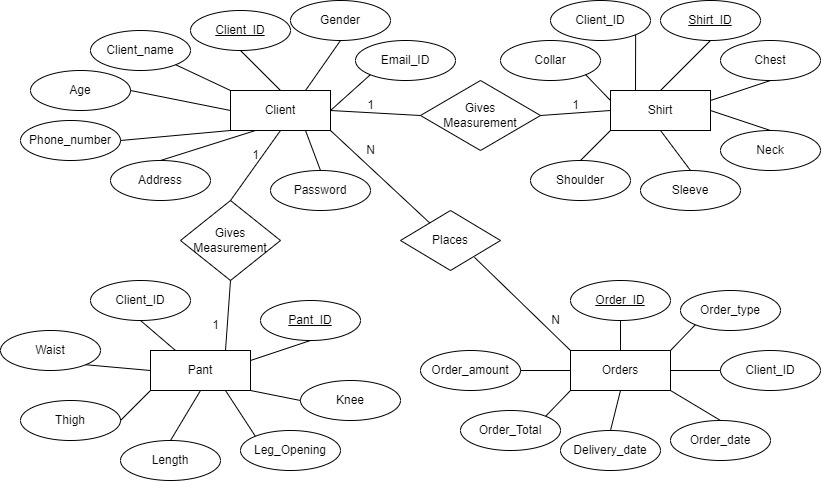
\includegraphics[width=1\textwidth]{tailor_database.jpg}
 \caption{ER diagram}
 \label{fig:tailor_database.jpg}
\end{figure}
\\
\\
\\
\\
\\
\\
\\
\\
\section{Schema Diagram} 
Figure:\ref{fig:tailor_schema(1).jpg} shows the Schema Diagram of Tailor's Database.
\\
\\
\\
\begin{figure}[h]
 \centering
 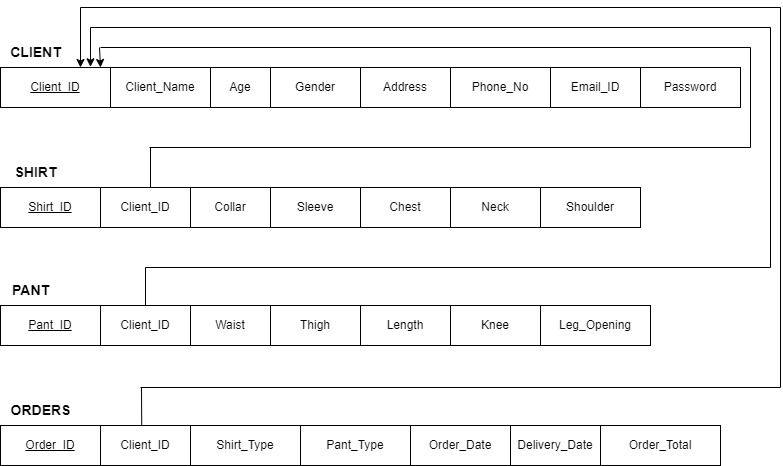
\includegraphics[width=1\textwidth]{tailor_schema (1).jpg}
 \caption{Schema diagram}
 \label{fig:tailor_schema(1).jpg}
\end{figure}
\section{Table description} 
\begin{center}
\begin{table}[h!]
\centering
    \begin{tabular}{|c|c|c|c|}
    \hline
      Attributes &Datatype &Constraints&Description  \\
      \hline
      \hline
         CLIENT-ID&INT&PRIMARY KEY&ID of client  \\
         \hline
         CLIENT-NAME&VARCHAR&NOT NULL& Name of the client\\ 
         \hline
         AGE&INT&NOT NULL& Client's age\\ 
         \hline
         GENDER&VARCHAR&NOT NULL&Client's gender\\
         \hline
         ADDRESS&TEXT&NOT NULL&Client's address\\
         \hline
         PH-NO&BIGINT&NOT NULL&Client's phone number\\
         \hline
         EMAIL-ID&VARCHAR&NOT NULL&Client's email id\\
         \hline
         PASSWORD&VARCHAR&NOT NULL&Client's password\\
         \hline
    \end{tabular}
    \caption{Client details .}
\label{table:1}
    \end{table}
\end{center}

\begin{center}
\begin{table}[h!]
\centering
    \begin{tabular}{|c|c|c|c|}
    \hline
      Attributes &Datatype &Constraints&Description  \\
      \hline
      \hline
         SHIRT-ID&INT&PRIMARY KEY&ID of shirt  \\
         \hline
         CLIENT-ID&INT&FOREIGN KEY&ID of client\\
         \hline
         COLLAR&FLOAT&NOT NULL& Collar size\\ 
         \hline
         SLEEVE&FLOAT&NOT NULL& Length of the sleeve\\ 
         \hline
         CHEST&FLOAT&NOT NULL& Chest's measurement\\
         \hline
         NECK&FLOAT&NOT NULL&Neck to shoulder size\\
         \hline
         SHOULDER&FLOAT&NOT NULL&Shoulder to shoulder length\\
         \hline
    \end{tabular}
    \caption{Shirt Table.}
\label{table:2}
    \end{table}
\end{center}

\begin{center}
\begin{table}[h!]
\centering
    \begin{tabular}{|c|c|c|c|}
    \hline
      Attributes &Datatype &Constraints&Description  \\
      \hline
      \hline
         PANT-ID&INT&PRIMARY KEY&ID of pant  \\
         \hline
         CLIENT-ID&INT&FOREIGN KEY&ID of client\\
         \hline
         WAIST&FLOAT&NOT NULL& Waist size\\ 
         \hline
         THIGH&FLOAT&NOT NULL& Thigh length\\ 
         \hline
         LENGTH&FLOAT&NOT NULL& Length of the pant\\
         \hline
         KNEE&FLOAT&NOT NULL&Knee size\\
         \hline
         LEG-OPENING&FLOAT&NOT NULL&Width of the cuff\\
         \hline
    \end{tabular}
    \caption{Pant Table.}
\label{table:3}
    \end{table}
\end{center}

\begin{center}
\begin{table}[h!]
\centering
    \begin{tabular}{|c|c|c|c|}
    \hline
      Attributes &Datatype &Constraints&Description  \\
      \hline
      \hline
         ORDER-ID&INT&PRIMARY KEY&ID of order \\
         \hline
         CLIENT-ID&INT&FOREIGN KEY&ID of client\\
         \hline
         SHIRT-TYPE&VARCHAR&NULL& Type of shirt\\ 
         \hline
         PANT-TYPE&VARCHAR&NULL& Type of pant\\ 
         \hline
         ORDER-DATE&DATE&NULL& Date of order\\
         \hline
         DELIVERY-DATE&DATE&NULL&Date of delivery\\
         \hline
         ORDER-TOTAL&DECIMAL&NULL&Total order amount\\
         \hline
    \end{tabular}
    \caption{Orders Table.}
\label{table:4}
    \end{table}
\end{center}

\chapter{Screenshots}

Figure:\ref{fig:HomePage.jpeg} shows the screenshot of home page 
\begin{figure}[h]
 \centering
 
\includegraphics[width=0.75\textwidth]{HomePage.jpeg}
 \caption{Home Page}
 \label{fig:HomePage.jpeg}
\end{figure}
\\
\\
\\
Figure:\ref{fig:signup.jpeg} shows the screenshot of sign up page
\begin{figure}[h]
 \centering
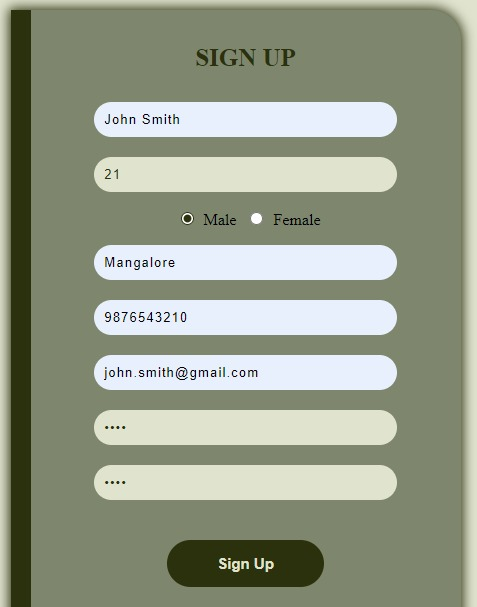
\includegraphics[width=0.75\textwidth,height=0.5\textwidth]{signup.jpeg}
 \caption{Sign Up Page}
 \label{fig:signup.jpeg}
\end{figure}
\\
\\
Figure:\ref{fig:PersonalDetails.jpeg} shows the screenshot of personal details page
\begin{figure}[h]
 \centering
 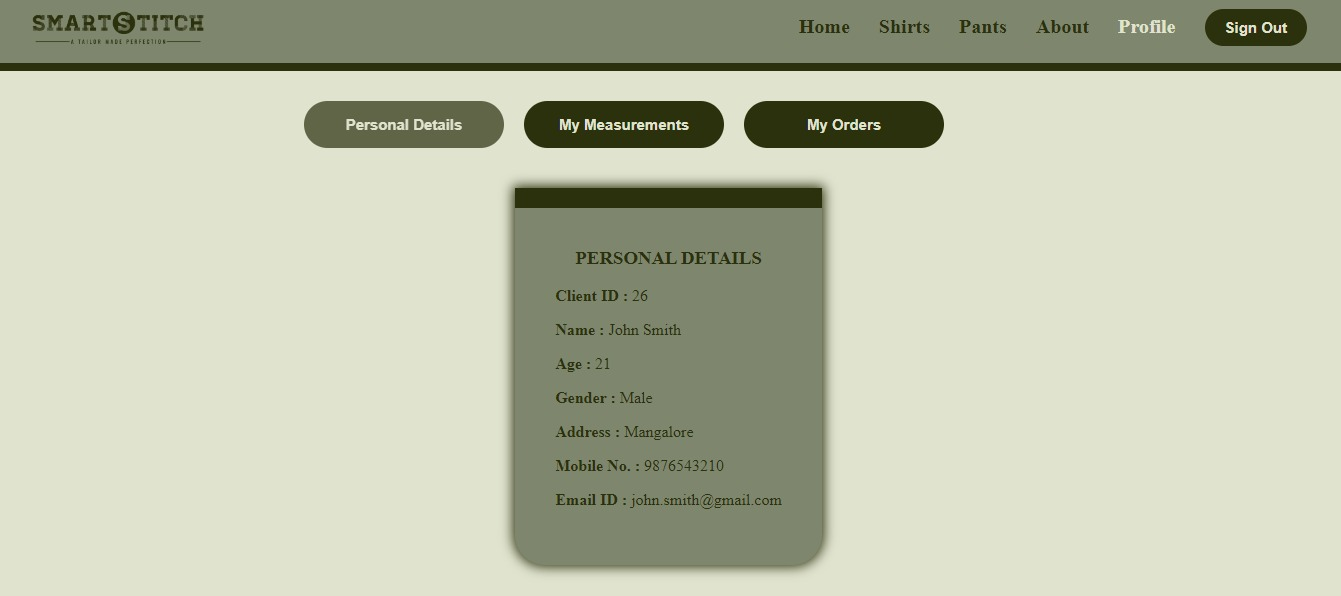
\includegraphics[width=0.75\textwidth]{PersonalDetails.jpeg}
 \caption{Personal Details Page}
 \label{fig:PersonalDetails.jpeg}
\end{figure}
\\
\\
Figure:\ref{fig:Measurements.jpeg} shows the screenshot of measurement details page
\begin{figure}[h]
 \centering
 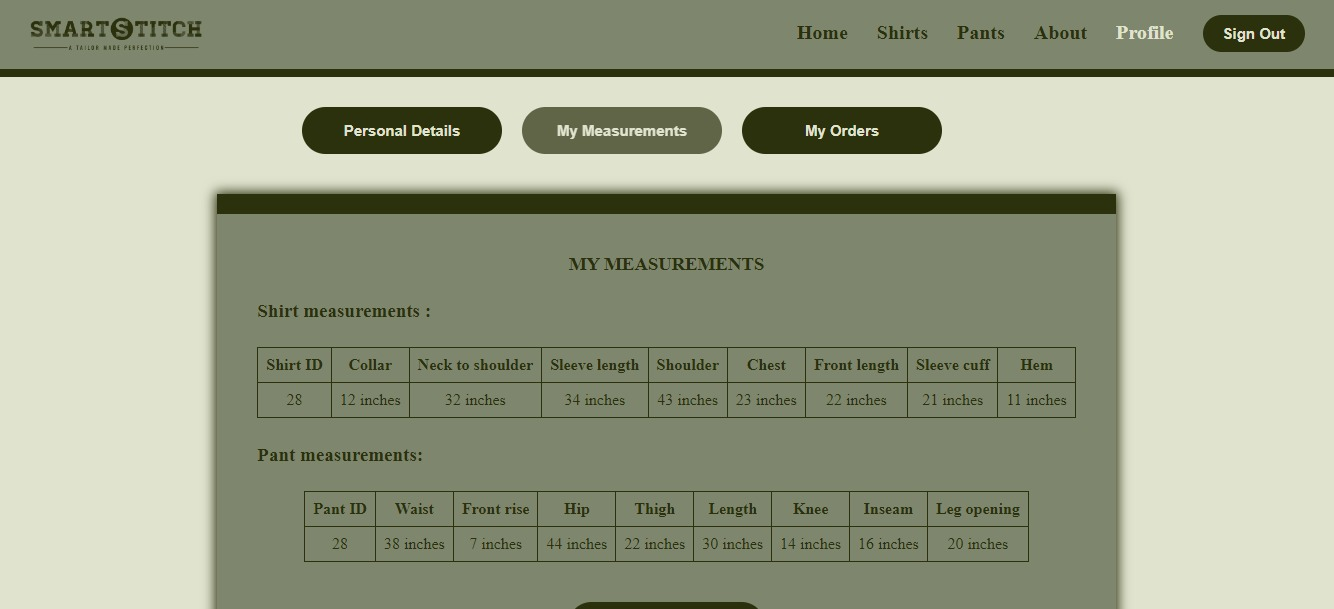
\includegraphics[width=0.75\textwidth]{Measurements.jpeg}
 \caption{Measurement Details Page}
 \label{fig:Measurements.jpeg}
\end{figure}
\\
\\
Figure:\ref{fig:Shirt_and_Pant.jpeg} shows the screenshot of shirt and pant details page
\begin{figure}[h!]
 \centering
 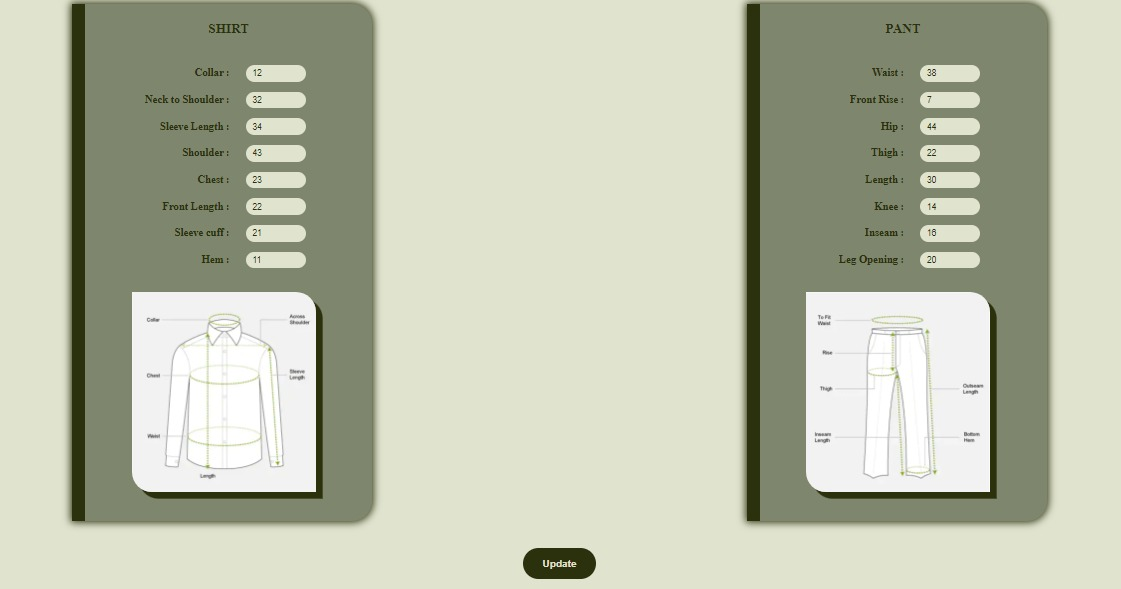
\includegraphics[width=0.75\textwidth]{Shirt_and_Pant.jpeg}
 \caption{Shirt and Pant Details Page}
 \label{fig:Shirt_and_Pant.jpeg}
\end{figure}
\\
\chapter{Conclusion and Future Scope}

\textbf{Conclusion} 
\begin{spacing}{1.5}
\begin{itemize}
 \item {In conclusion, the Tailor's Database Management System (DBMS) project offers numerous benefits for tailor shops by streamlining operations, improving customer service, and providing valuable insights for business growth. By effectively managing customer information, orders, inventory, and financial data, the DBMS enhances efficiency, accuracy, and customer satisfaction.}
 \item {The project's successful implementation involves careful planning, database design, user-friendly interfaces, and robust security measures. Regular maintenance and support are essential to ensure the system's continued effectiveness.}
\end{itemize}
\textbf{Future Scope} 
\begin{itemize}
 \item {\textbf{Integration with E-commerce}: As online shopping and custom clothing services become more popular, integrating the DBMS with an e-commerce platform can expand the tailor shop's reach and customer base.}

\item{\textbf{Mobile Application}: Develop a mobile app for customers to schedule appointments, track orders, and communicate with the tailor shop conveniently.}

\item{\textbf{Machine Learning and AI}: Implement AI-driven features for trend analysis, size recommendations, and personalized style suggestions based on customer data.}

\item{\textbf{Multi-location Support}: If the tailor shop expands to multiple locations, the DBMS can be extended to support centralized management of all branches.}

\item{\textbf{Customer Feedback and Reviews}: Include features for customers to provide feedback and reviews, helping the tailor shop improve its services and reputation.}
\end{itemize}
\end{spacing}

\begin{thebibliography}{7}
\addcontentsline{toc}{chapter}{References}
\begin{spacing}{1.5}
    \bibitem{texbook}
Adebola Omopariola (May 2023)\emph{ Design and Implementation of a Tailoring Management System (Virlor)}, Veritas University Abuja.

\bibitem{textbook}
 Jagdish Chandra Patni, Hitesh Kumar Sharma, Ravi Tomar, Avita Katal (January 27, 2022) \emph{Database Management System
An Evolutionary Approach}, CRC Press,1st Edition

\bibitem{texbook}
Marko Rosenmuller, Sven Apel (December 2009)\emph{ Tailor-made data management for embedded systems}, Data and Knowledge Engineering, Volume 68, 2009.

\bibitem{texbook}
 Raghu Ramakrishnan, Johannes Gehrke(14 August 2002)\emph{ Database Management Systems}, McGraw-Hill, Inc., Professional Book Group 11 West 19th Street New York, NY, United States
\end{spacing}
\end{thebibliography}


\end{document}